\documentclass{standalone}
\usepackage{tikz}
\usetikzlibrary{patterns, positioning}


\begin{document}
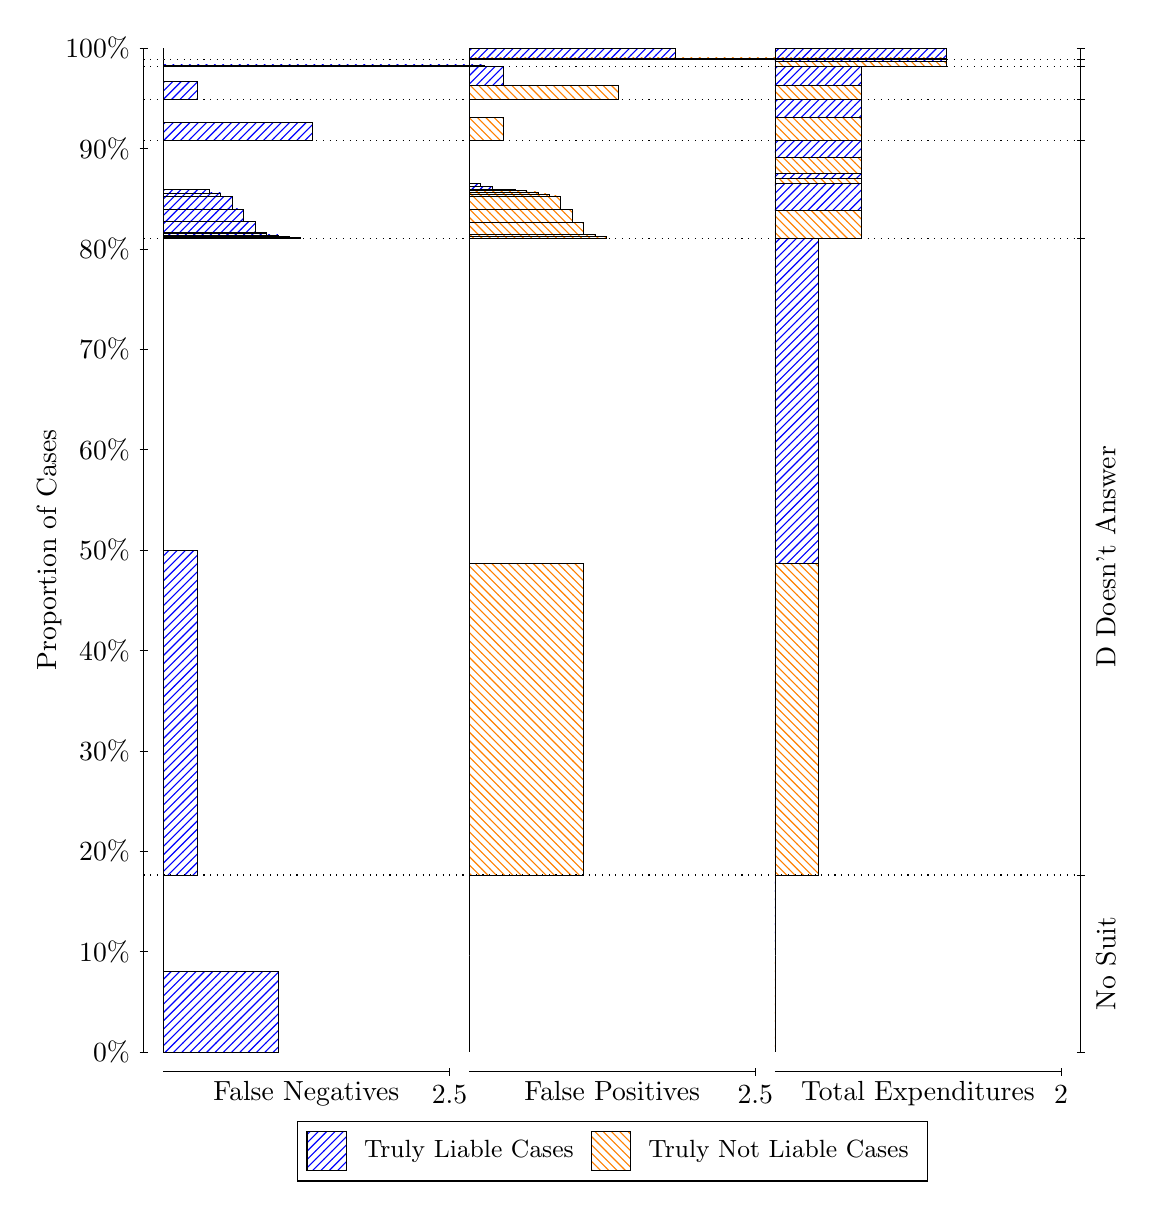
\begin{tikzpicture}
\draw[black, very thin] (1.5,1.75) -- (1.5,14.5);
\node[rotate=90, text=black, anchor=center] at (0.3, 8.125) {Proportion of Cases};
\draw[black, very thin] (1.45,1.75) -- (1.55,1.75);
\node[text=black, anchor=east] at (1.45, 1.75) {0\%};
\draw[black, very thin] (1.45,3.025) -- (1.55,3.025);
\node[text=black, anchor=east] at (1.45, 3.025) {10\%};
\draw[black, very thin] (1.45,4.3) -- (1.55,4.3);
\node[text=black, anchor=east] at (1.45, 4.3) {20\%};
\draw[black, very thin] (1.45,5.575) -- (1.55,5.575);
\node[text=black, anchor=east] at (1.45, 5.575) {30\%};
\draw[black, very thin] (1.45,6.85) -- (1.55,6.85);
\node[text=black, anchor=east] at (1.45, 6.85) {40\%};
\draw[black, very thin] (1.45,8.125) -- (1.55,8.125);
\node[text=black, anchor=east] at (1.45, 8.125) {50\%};
\draw[black, very thin] (1.45,9.4) -- (1.55,9.4);
\node[text=black, anchor=east] at (1.45, 9.4) {60\%};
\draw[black, very thin] (1.45,10.675) -- (1.55,10.675);
\node[text=black, anchor=east] at (1.45, 10.675) {70\%};
\draw[black, very thin] (1.45,11.95) -- (1.55,11.95);
\node[text=black, anchor=east] at (1.45, 11.95) {80\%};
\draw[black, very thin] (1.45,13.225) -- (1.55,13.225);
\node[text=black, anchor=east] at (1.45, 13.225) {90\%};
\draw[black, very thin] (1.45,14.5) -- (1.55,14.5);
\node[text=black, anchor=east] at (1.45, 14.5) {100\%};

\draw[black, very thin] (13.4,1.75) -- (13.4,14.5);
\draw[black, very thin] (13.35,1.75) -- (13.45,1.75);
\node[anchor=west] at (13.35, 1.75) {};
\draw[black, very thin] (13.35,3.997) -- (13.45,3.997);
\node[anchor=west] at (13.35, 3.997) {};
\draw[black, very thin] (13.35,12.079) -- (13.45,12.079);
\node[anchor=west] at (13.35, 12.079) {};
\draw[black, very thin] (13.35,13.324) -- (13.45,13.324);
\node[anchor=west] at (13.35, 13.324) {};
\draw[black, very thin] (13.35,13.843) -- (13.45,13.843);
\node[anchor=west] at (13.35, 13.843) {};
\draw[black, very thin] (13.35,14.266) -- (13.45,14.266);
\node[anchor=west] at (13.35, 14.266) {};
\draw[black, very thin] (13.35,14.353) -- (13.45,14.353);
\node[anchor=west] at (13.35, 14.353) {};
\draw[black, very thin] (13.35,14.5) -- (13.45,14.5);
\node[anchor=west] at (13.35, 14.5) {};

\draw[black, very thin, pattern color=blue, pattern=north east lines] (1.75,1.75) rectangle (3.2033,2.7703);
\draw[black, very thin, pattern color=orange, pattern=north west lines] (1.75,2.7703) rectangle (1.75,3.997);
\draw[black, very thin, pattern color=blue, pattern=north east lines] (1.75,3.997) rectangle (2.186,8.1171);
\draw[black, very thin, pattern color=orange, pattern=north west lines] (1.75,8.1171) rectangle (1.75,12.079);
\draw[black, very thin, pattern color=blue, pattern=north east lines] (1.75,12.079) rectangle (3.494,12.091);
\draw[black, very thin, pattern color=blue, pattern=north east lines] (1.75,12.091) rectangle (3.3487,12.103);
\draw[black, very thin, pattern color=blue, pattern=north east lines] (1.75,12.103) rectangle (3.2033,12.128);
\draw[black, very thin, pattern color=blue, pattern=north east lines] (1.75,12.128) rectangle (3.058,12.143);
\draw[black, very thin, pattern color=blue, pattern=north east lines] (1.75,12.143) rectangle (3.058,12.156);
\draw[black, very thin, pattern color=blue, pattern=north east lines] (1.75,12.156) rectangle (2.9127,12.297);
\draw[black, very thin, pattern color=blue, pattern=north east lines] (1.75,12.297) rectangle (2.7673,12.456);
\draw[black, very thin, pattern color=blue, pattern=north east lines] (1.75,12.456) rectangle (2.622,12.619);
\draw[black, very thin, pattern color=blue, pattern=north east lines] (1.75,12.619) rectangle (2.4767,12.659);
\draw[black, very thin, pattern color=blue, pattern=north east lines] (1.75,12.659) rectangle (2.3313,12.702);
\draw[black, very thin, pattern color=orange, pattern=north west lines] (1.75,12.702) rectangle (1.75,13.324);
\draw[black, very thin, pattern color=blue, pattern=north east lines] (1.75,13.324) rectangle (3.6393,13.552);
\draw[black, very thin, pattern color=orange, pattern=north west lines] (1.75,13.552) rectangle (1.75,13.843);
\draw[black, very thin, pattern color=blue, pattern=north east lines] (1.75,13.843) rectangle (2.186,14.08);
\draw[black, very thin, pattern color=orange, pattern=north west lines] (1.75,14.08) rectangle (1.75,14.266);
\draw[black, very thin, pattern color=blue, pattern=north east lines] (1.75,14.266) rectangle (5.8193,14.286);
\draw[black, very thin, pattern color=orange, pattern=north west lines] (1.75,14.286) rectangle (1.75,14.353);
\draw[black, very thin, pattern color=orange, pattern=north west lines] (1.75,14.353) rectangle (1.75,14.374);
\draw[black, very thin, pattern color=blue, pattern=north east lines] (1.75,14.374) rectangle (1.75,14.5);
\draw[black, very thin, pattern color=orange, pattern=north west lines] (5.6333,1.75) rectangle (5.6333,2.9767);
\draw[black, very thin, pattern color=blue, pattern=north east lines] (5.6333,2.9767) rectangle (5.6333,3.997);
\draw[black, very thin, pattern color=orange, pattern=north west lines] (5.6333,3.997) rectangle (7.0867,7.9584);
\draw[black, very thin, pattern color=blue, pattern=north east lines] (5.6333,7.9584) rectangle (5.6333,12.079);
\draw[black, very thin, pattern color=orange, pattern=north west lines] (5.6333,12.079) rectangle (7.3773,12.105);
\draw[black, very thin, pattern color=orange, pattern=north west lines] (5.6333,12.105) rectangle (7.232,12.132);
\draw[black, very thin, pattern color=orange, pattern=north west lines] (5.6333,12.132) rectangle (7.0867,12.288);
\draw[black, very thin, pattern color=orange, pattern=north west lines] (5.6333,12.288) rectangle (6.9413,12.447);
\draw[black, very thin, pattern color=orange, pattern=north west lines] (5.6333,12.447) rectangle (6.796,12.621);
\draw[black, very thin, pattern color=orange, pattern=north west lines] (5.6333,12.621) rectangle (6.6507,12.647);
\draw[black, very thin, pattern color=orange, pattern=north west lines] (5.6333,12.647) rectangle (6.5053,12.674);
\draw[black, very thin, pattern color=orange, pattern=north west lines] (5.6333,12.674) rectangle (6.36,12.688);
\draw[black, very thin, pattern color=orange, pattern=north west lines] (5.6333,12.688) rectangle (6.2147,12.701);
\draw[black, very thin, pattern color=blue, pattern=north east lines] (5.6333,12.701) rectangle (5.924,12.743);
\draw[black, very thin, pattern color=blue, pattern=north east lines] (5.6333,12.743) rectangle (5.7787,12.784);
\draw[black, very thin, pattern color=blue, pattern=north east lines] (5.6333,12.784) rectangle (5.6333,13.324);
\draw[black, very thin, pattern color=orange, pattern=north west lines] (5.6333,13.324) rectangle (6.0693,13.615);
\draw[black, very thin, pattern color=blue, pattern=north east lines] (5.6333,13.615) rectangle (5.6333,13.843);
\draw[black, very thin, pattern color=orange, pattern=north west lines] (5.6333,13.843) rectangle (7.5227,14.029);
\draw[black, very thin, pattern color=blue, pattern=north east lines] (5.6333,14.029) rectangle (6.0693,14.266);
\draw[black, very thin, pattern color=orange, pattern=north west lines] (5.6333,14.266) rectangle (5.6333,14.333);
\draw[black, very thin, pattern color=blue, pattern=north east lines] (5.6333,14.333) rectangle (5.6333,14.353);
\draw[black, very thin, pattern color=orange, pattern=north west lines] (5.6333,14.353) rectangle (9.7027,14.374);
\draw[black, very thin, pattern color=blue, pattern=north east lines] (5.6333,14.374) rectangle (8.2493,14.5);
\draw[black, very thin, pattern color=orange, pattern=north west lines] (9.5167,1.75) rectangle (9.5167,2.9767);
\draw[black, very thin, pattern color=blue, pattern=north east lines] (9.5167,2.9767) rectangle (9.5167,3.997);
\draw[black, very thin, pattern color=orange, pattern=north west lines] (9.5167,3.997) rectangle (10.062,7.9584);
\draw[black, very thin, pattern color=blue, pattern=north east lines] (9.5167,7.9584) rectangle (10.062,12.079);
\draw[black, very thin, pattern color=orange, pattern=north west lines] (9.5167,12.079) rectangle (10.607,12.435);
\draw[black, very thin, pattern color=blue, pattern=north east lines] (9.5167,12.435) rectangle (10.607,12.781);
\draw[black, very thin, pattern color=orange, pattern=north west lines] (9.5167,12.781) rectangle (10.607,12.847);
\draw[black, very thin, pattern color=blue, pattern=north east lines] (9.5167,12.847) rectangle (10.607,12.912);
\draw[black, very thin, pattern color=orange, pattern=north west lines] (9.5167,12.912) rectangle (10.607,13.111);
\draw[black, very thin, pattern color=blue, pattern=north east lines] (9.5167,13.111) rectangle (10.607,13.324);
\draw[black, very thin, pattern color=orange, pattern=north west lines] (9.5167,13.324) rectangle (10.607,13.615);
\draw[black, very thin, pattern color=blue, pattern=north east lines] (9.5167,13.615) rectangle (10.607,13.843);
\draw[black, very thin, pattern color=orange, pattern=north west lines] (9.5167,13.843) rectangle (10.607,14.029);
\draw[black, very thin, pattern color=blue, pattern=north east lines] (9.5167,14.029) rectangle (10.607,14.266);
\draw[black, very thin, pattern color=orange, pattern=north west lines] (9.5167,14.266) rectangle (11.697,14.333);
\draw[black, very thin, pattern color=blue, pattern=north east lines] (9.5167,14.333) rectangle (11.697,14.353);
\draw[black, very thin, pattern color=orange, pattern=north west lines] (9.5167,14.353) rectangle (11.697,14.374);
\draw[black, very thin, pattern color=blue, pattern=north east lines] (9.5167,14.374) rectangle (11.697,14.5);
\draw[black, dotted] (1.5,3.997) -- (13.4,3.997);
\draw[black, dotted] (1.5,12.079) -- (13.4,12.079);
\draw[black, dotted] (1.5,13.324) -- (13.4,13.324);
\draw[black, dotted] (1.5,13.843) -- (13.4,13.843);
\draw[black, dotted] (1.5,14.266) -- (13.4,14.266);
\draw[black, dotted] (1.5,14.353) -- (13.4,14.353);
\draw[black, very thin] (1.75,1.5) -- (5.3833,1.5);
\node[text=black, anchor=north] at (3.5667, 1.5) {False Negatives};
\draw[black, very thin] (5.3833,1.45) -- (5.3833,1.55);
\node[text=black, anchor=north] at (5.3833, 1.45) {2.5};

\draw[black, very thin] (5.6333,1.5) -- (9.2667,1.5);
\node[text=black, anchor=north] at (7.45, 1.5) {False Positives};
\draw[black, very thin] (9.2667,1.45) -- (9.2667,1.55);
\node[text=black, anchor=north] at (9.2667, 1.45) {2.5};

\draw[black, very thin] (9.5167,1.5) -- (13.15,1.5);
\node[text=black, anchor=north] at (11.333, 1.5) {Total Expenditures};
\draw[black, very thin] (13.15,1.45) -- (13.15,1.55);
\node[text=black, anchor=north] at (13.15, 1.45) {2};

\node[text=black, centered, rotate=90] at (13.72, 2.8735) {No Suit};
\node[text=black, centered, rotate=90] at (13.72, 8.0377) {D Doesn't Answer};






\draw (7.449999999999999,1.5) node[draw=none] (baseCoordinate) {};
\begin{scope}[align=center]
        \matrix[scale=0.5, draw=black, below=0.5cm of baseCoordinate, nodes={draw}, column sep=0.1cm]{
            \node[rectangle, draw, minimum width=0.5cm, minimum height=0.5cm, pattern color=blue, pattern=north east lines] {}; &
            \node[draw=none, font=\small, text=black] (B) {Truly Liable Cases}; &
            \node[rectangle, draw, minimum width=0.5cm, minimum height=0.5cm, pattern color=orange, pattern=north west lines] {}; &
            \node[draw=none, font=\small, text=black] (B) {Truly Not Liable Cases}; \\
            };
\end{scope}

\end{tikzpicture}
\end{document}